\documentclass[tikz,border=6pt]{standalone}

\usepackage{tikz}

\begin{document}
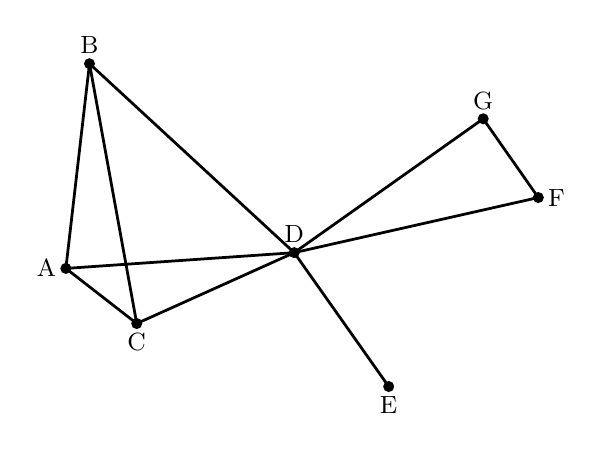
\begin{tikzpicture}[x=1cm,y=1cm, line cap=round, line join=round, font=\small]

% ============================================================
% A) THAM SỐ HÓA (đổi ở đây)
% ============================================================
% Khung (chỉ để canh bố cục; không vẽ khung)
\def\W{8.4}
\def\H{5.8}

% Tọa độ các đỉnh (chọn để giống hình)
\def\Ax{1.1}\def\Ay{2.2}
\def\Bx{1.4}\def\By{4.8}
\def\Cx{2.0}\def\Cy{1.5}
\def\Dx{4.0}\def\Dy{2.4}
\def\Ex{5.2}\def\Ey{0.7}
\def\Fx{7.1}\def\Fy{3.1}
\def\Gx{6.4}\def\Gy{4.1}

% Kích thước điểm
\def\rPt{2.0pt}

% ============================================================
% B) ĐỊNH NGHĨA ĐIỂM
% ============================================================
\coordinate (A) at (\Ax,\Ay);
\coordinate (B) at (\Bx,\By);
\coordinate (C) at (\Cx,\Cy);
\coordinate (D) at (\Dx,\Dy);
\coordinate (E) at (\Ex,\Ey);
\coordinate (F) at (\Fx,\Fy);
\coordinate (G) at (\Gx,\Gy);

% ============================================================
% C) CẠNH (đúng cấu trúc hình)
% ============================================================
% Cụm trái
\draw[line width=1.0pt] (B)--(A);
\draw[line width=1.0pt] (A)--(C);
\draw[line width=1.0pt] (A)--(D);
\draw[line width=1.0pt] (B)--(C);
\draw[line width=1.0pt] (B)--(D);
\draw[line width=1.0pt] (C)--(D);

% Nhánh xuống E
\draw[line width=1.0pt] (D)--(E);

% Cụm phải
\draw[line width=1.0pt] (D)--(F);
\draw[line width=1.0pt] (D)--(G);
\draw[line width=1.0pt] (G)--(F);

% ============================================================
% D) ĐIỂM + NHÃN
% ============================================================
\foreach \P/\pos in {A/left,B/above,C/below,D/above,E/below,F/right,G/above}{
  \fill (\P) circle (\rPt);
  \node[\pos] at (\P) {\P};
}

\end{tikzpicture}
\end{document}
